\documentclass[11pt]{article}
\usepackage{charter}
\usepackage{graphicx}
\usepackage{hyperref}
\usepackage{mdframed}
\usepackage[margin=1in]{geometry}
\usepackage{amsmath}

\hypersetup{
	colorlinks=true,
	linkcolor=blue,
	filecolor=magenta,
	urlcolor=cyan,
}

\begin{document}

%===================================================
% Title and Author Info
%===================================================
\begin{center}
{\Large\textsc{Relativistic Orbits}} \\
\vspace{10pt}
{\large \textbf{Mentor:} Alex Urban} \\
{\small LIGO Laboratory, California Institute of Technology \\
Pasadena, CA 91125, USA \\
\href{mailto:aurban@ligo.caltech.edu}{\texttt{aurban@ligo.caltech.edu}}}
\end{center}

%%%%%%%%%%%%%%%%%%%%%%%%%%%%%%%%%%%%%%%%%%%%%%%%%%%

\section*{Purpose}

\hspace{15pt} In this problem set, we will try out a better numerical integration scheme, then work out the total energy of a ``simple'' relativistic orbit and simulate it in Python. We will also look at a fun toy problem that starts to get at the dynamics that lead to electromagnetic counterparts of compact binary mergers. The goal is to start putting together all the astrophysics we've been learning in an awesome relativistic orbit simulation.... \textit{of science!}

\section*{Relativistic Orbits in a Simple Curved Spacetime}
\hspace{15pt} Suppose that a neutron star binary (each with mass $M = 1.4\,\, M_{\odot}$) is in a stable orbit, still with no loss of energy, but now in Schwarzschild spacetime. Figure \ref{fig:binary_diagram} illustrates this system.

\vspace{20pt}

\begin{figure}[!h]
\begin{mdframed}
\centering
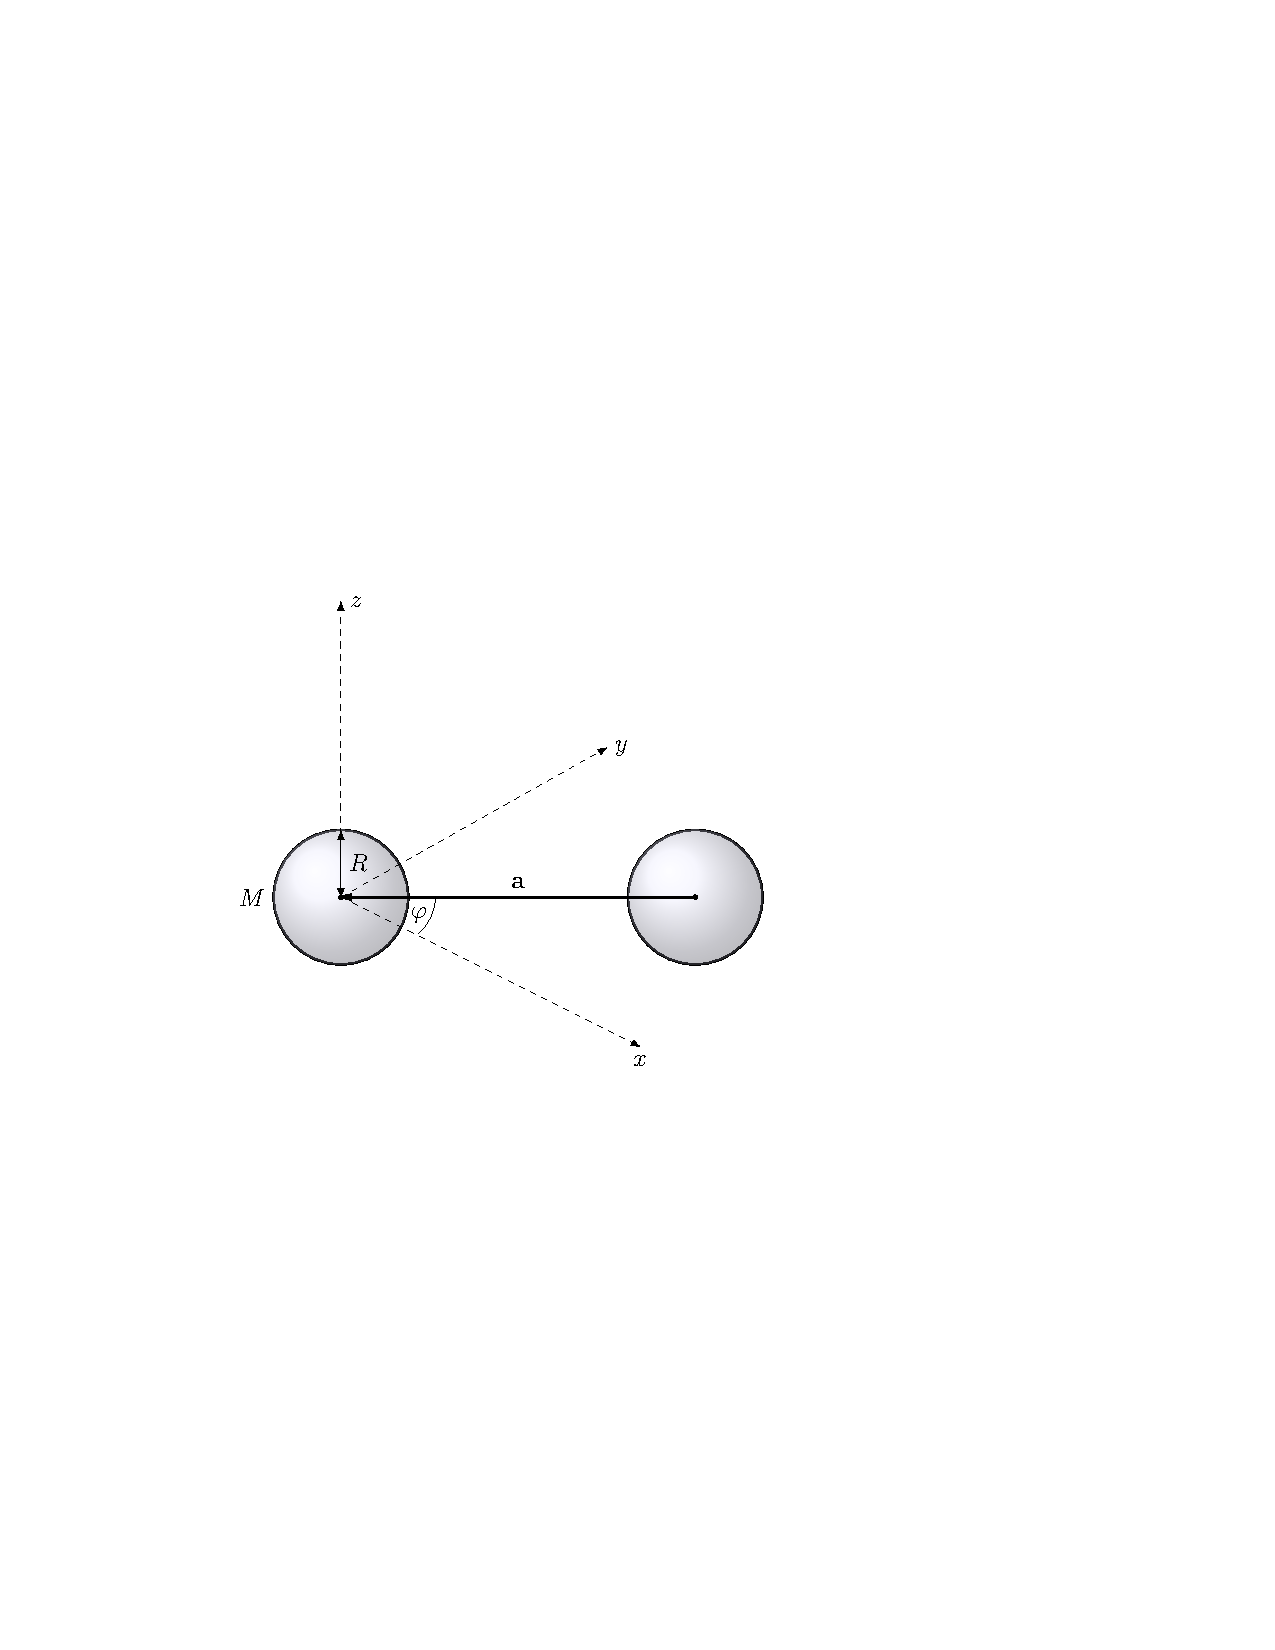
\includegraphics{relativistic_orbit/binary_diagram.pdf}
\caption{\label{fig:binary_diagram}Diagram of the neutron star binary in the rest frame of star 1, showing its orbital separation vector ($\mathbf{r}$) and the radius ($R$) and masses ($m_1$, $m_2$) of the individual neutron stars. The azimuthal angle $\varphi$ is also indicated.}
\end{mdframed}
\end{figure}

\vspace{1000pt}

\begin{enumerate}

\item First, we want to experiment with a better numerical integrator using a problem we already understand. Try re-doing the Keplerian orbit simulation, only this time, use the RK4 integration scheme: if $t_i, \dots, t_N$ are a series of time samples and $df/dt = g(f, t)$ a differential equation for some set of functions $f$, then the RK4 method
\begin{align*}
k_1 &= g(f(t_i), \, t_i) \\
k_2 &= g\left(f(t_i) + \frac{hk_1}{2}, \, t_i + \frac{h}{2}\right) \\
k_3 &= g\left(f(t_i) + \frac{hk_2}{2}, \, t_i + \frac{h}{2}\right) \\
k_4 &= g(f(t_i) + hk_3, \, t_i + h) \\
f(t_{i+1}) &= f(t_i) + \frac{h}{6}\,\left(k_1 + 2k_2 + 2k_3 + k_4\right)
\end{align*}
is a generalization of Simpson's rule with step size $h$.

\hspace{15pt} Show that, for the Keplerian orbit problem, the RK4 method still conserves energy and angular momentum, and that it allows you to use a much larger step size without introducing numerical error. (How much larger can the step size be?)

\item To visualize some important effects from general relativity, consider a correction to the total energy that comes from the simplest example of curved spacetime:
\begin{equation}
\frac{E^2 - \mu c^2}{2\mu c^2} = \frac{1}{2}\mu\left(\frac{dr}{d\tau}\right)^2 + \Phi(r, L)
\end{equation}
where $\tau$ is the proper time, $\mu = m_1 m_2/(m_1 + m_2)$ is the reduced mass, $M = m_1 + m_2$ is the total mass, and the effective potential
\begin{equation}\label{eq:potential}
\Phi(r, L) = -\frac{GM\mu}{r} + \frac{L^2}{2\mu r^2} - \frac{GML^2}{c^2\mu r^3}
\end{equation}
now has an extra attractive centrifugal term. Using what you know about calculus and circular orbits, show that with this potential there can be no stable circular orbits closer than a radius
\begin{equation}\label{eq:ISCO}
r_{\rm ISCO} = \frac{6GM}{c^2}.
\end{equation}
In astrophysics jargon, this is called the ISCO radius (short for Innermost Stable Circular Orbit). What is $r_{\rm ISCO}$ as a function of gravitational wave frequency?

\item Perform a simulation of orbits in this spacetime, using masses of 1.4 $M_{\odot}$ for each body and experimenting with different initial conditions. What angular momenta do you need to visualize ISCO properties? If you use RK4, is the total (relativistic) energy conserved?

\item Finally, let's have some fun with a toy problem that works as a surprisingly good model for the physics of $\gamma$-ray bursts: the relativistic cannonball. Suppose a cannonball of mass $m_1$ moving at Lorentz factor $\Gamma$ collides with another particle of mass $m_2$ that is initially at rest.
\begin{enumerate}
\item To a very distant observer watching this epic lightshow (at rest), what is the time between the muzzle flash of the cannon and the collision of the masses? Write this in terms of the time as measured in the rest frame of $m_1$.

\item If the collision is completely inelastic (so that the masses stick together), use the conservation of 4-momentum to find the final energy and momentum, and write the final Lorentz factor in terms of the mass ratio $m_1/m_2$.
\end{enumerate}

\end{enumerate}

%%%%%%%%%%%%%%%%%%%%%%%%%%%%%%%%%%%%%%%%%%%%%%%%%%%

\section*{Things That Make You Go, ``Hmmm....''}

\begin{enumerate}

\item How much energy is available at the ISCO radius to power gravitational radiation and $\gamma$-ray bursts?

\item What does your figure for $m_1/m_2$ in the last problem tell us about the mass of the disk that forms during compact binary mergers? Full disclosure: this is not a trick question, but it's also not an easy one. There is a lot of physics that goes into answering this, but I want you to try mulling it over. Don't be afraid to use tools like google; in fact, doing a literature search is generally always a great thing to do when you want to understand something new!

\item Suppose we add to the Keplerian system a tiny point particle of mass $m \ll M$. What do you think its motion would look like in different regions?

\end{enumerate}

%%%%%%%%%%%%%%%%%%%%%%%%%%%%%%%%%%%%%%%%%%%%%%%%%%%

\vspace{1000pt}

%%%%%%%%%%%%%%%%%%%%%%%%%%%%%%%%%%%%%%%%%%%%%%%%%%%

\subsection*{Solution}

\begin{enumerate}

\item 

\item 

\item 

\item 

\end{enumerate}

%%%%%%%%%%%%%%%%%%%%%%%%%%%%%%%%%%%%%%%%%%%%%%%%%%%

\begin{mdframed}

\section*{Things That Make You Go, ``Hmmm....''}

\begin{enumerate}

\item How much energy is available at the ISCO radius to power gravitational radiation and $\gamma$-ray bursts?

\item What does your figure for $m_1/m_2$ in the last problem tell us about the mass of the disk that forms during compact binary mergers? Full disclosure: this is not a trick question, but it's also not an easy one. There is a lot of physics that goes into answering this, but I want you to try mulling it over. Don't be afraid to use tools like google; in fact, doing a literature search is generally always a great thing to do when you want to understand something new!

\item Suppose we add to the Keplerian system a tiny point particle of mass $m \ll M$. What do you think its motion would look like in different regions?

\end{enumerate}

\end{mdframed}

\end{document}
